\documentclass[12pt,a4paper,openany]{book}
\usepackage{lmodern}
\usepackage[svgnames]{xcolor} % Required to specify font color
\usepackage{xcolor}
\definecolor{vert1}{rgb}{0.0,0.3.9,0.0}
\definecolor{bleu}{rgb}{0,0,0.5}
\definecolor{bleu3}{rgb}{1,0.2,0.2}
\definecolor{grisgris}{gray}{0.4}
\definecolor{grisclair}{HTML}{E7E7E7}
\definecolor{grisfonce}{HTML}{A5A5A5}
\definecolor{rougeUPS}{rgb}{0.6, 0.3, 0.3}

\fboxsep =0pt \parindent =0pt\parskip =12pt



\usepackage[utf8]{inputenc} 
\usepackage[T1]{fontenc}
\usepackage{wrapfig}
\usepackage[francais]{babel}
\usepackage[top=1.7cm, bottom=1.7cm, left=1.7cm, right=1.7cm]{geometry}
\usepackage{verbatim}
\usepackage[urlbordercolor={1 1 1}, linkbordercolor={1 1 1}, linkcolor=vert1, urlcolor=bleu, colorlinks=true]{hyperref}
\usepackage{tikz} %Vectoriel
\usepackage{listings}
\usepackage{fancyhdr}
\usepackage{multido}
\usepackage{amssymb}
\usepackage{float}
\usepackage[francais]{minitoc}
\usepackage[final]{pdfpages} 
\usepackage{graphicx} % Required for box manipulation

\newcommand{\titre}{Traduction des langages}
\newcommand{\subtitle}{~}
\newcommand{\auteur}{Antoine de \bsc{Roquemaurel}}
\newcommand{\formation}{M1 Informatique -- Développement Logiciel}
\newcommand{\semestre}{7}
\newcommand{\annee}{2014}
\newcommand{\prof}{Christine \bsc{Maurel}}
\newcommand{\logo}{/home/aroquemaurel/cours/templates/templates/ups.jpg}


\newcommand{\pole}{}
\newcommand{\sigle}{TL}


\definecolor{gris1}{gray}{0.40}
\definecolor{gris2}{gray}{0.55}
\definecolor{gris3}{gray}{0.65}
\definecolor{gris4}{gray}{0.50}
\definecolor{vert}{rgb}{0,0.4,0}
\definecolor{violet}{rgb}{0.65, 0.2, 0.65}
\definecolor{bleu1}{rgb}{0,0,0.8}
\definecolor{bleu2}{rgb}{0,0.2,0.6}
\definecolor{bleu3}{rgb}{0,0.2,0.2}
\definecolor{rouge}{HTML}{F93928}


\lstdefinelanguage{algo}{%
   morekeywords={%
    %%% couleur 1
		importer, programme, glossaire, fonction, procedure, constante, type, 
	%%% IMPORT & Co.
		si, sinon, alors, fin, tantque, debut, faire, lorsque, fin lorsque, 
		declenche, declencher, enregistrement, tableau, retourne, retourner, =, pour, a,
		/=, <, >, traite,exception, 
	%%% types 
		Entier, Reel, Booleen, Caractere, Réél, Booléen, Caractère,
	%%% types 
		entree, maj, sortie,entrée,
	%%% types 
		et, ou, non,
	},
  sensitive=true,
  morecomment=[l]{--},
  morestring=[b]',
}

\lstset{language=algo,
    %%% BOUCLE, TEST & Co.
      emph={importer, programme, glossaire, fonction, procedure, constante, type},
      emphstyle=\color{bleu2},
    %%% IMPORT & Co.  
	emph={[2]
		si, sinon, alors, fin , tantque, debut, faire, lorsque, fin lorsque, 
		declencher, retourner, et, ou, non,enregistrement, retourner, retourne, 
		tableau, /=, <, =, >, traite,exception, pour, a
	},
      emphstyle=[2]\color{bleu1},
    %%% FONCTIONS NUMERIQUES
      emph={[3]Entier, Reel, Booleen, Caractere, Booléen, Réél, Caractère},
      emphstyle=[3]\color{gris1},
    %%% FONCTIONS NUMERIQUES
      emph={[4]entree, maj, sortie, entrée},	
      emphstyle=[4]\color{gris1},
}
\lstdefinelanguage{wl}{%
   morekeywords={%
    %%% couleur 1
		importer, programme, glossaire, fonction, procedure, constante, type, 
	%%% IMPORT & Co.
		si, sinon, alors, fin, TANTQUE, tantque, FIN, PROCEDURE, debut, faire, lorsque, 
		fin lorsque, declenche, declencher, enregistrement, tableau, retourne, retourner, =, 
		/=, <, >, traite,exception, 
	%%% types 
		Entier, Reel, Booleen, Caractere, Réél, Booléen, Caractère,
	%%% types 
		entree, maj, sortie,entrée,
	%%% types 
		et, ou, non,
	},
  sensitive=true,
  morecomment=[l]{//},
  morestring=[b]',
}

\lstset{language=wl,
    %%% BOUCLE, TEST & Co.
      emph={importer, programme, glossaire, fonction, procedure, constante, type},
      emphstyle=\color{bleu2},
    %%% IMPORT & Co.  
	emph={[2]
		si, sinon, alors, fin , tantque, debut, faire, lorsque, fin lorsque, 
		declencher, retourner, et, ou, non,enregistrement, retourner, retourne, 
		tableau, /=, <, =, >, traite,exception
	},
      emphstyle=[2]\color{bleu1},
    %%% FONCTIONS NUMERIQUES
      emph={[3]Entier, Reel, Booleen, Caractere, Booléen, Réél, Caractère},
      emphstyle=[3]\color{gris1},
    %%% FONCTIONS NUMERIQUES
      emph={[4]entree, maj, sortie, entrée},	
      emphstyle=[4]\color{gris1},
}
\lstdefinelanguage{css}{%
   morekeywords={%
    %%% couleur 1
		background, image, repeat, position, index, color, border, font, 
		size, url, family, style, variant, weight, letter, spacing, line, 
		height, text, decoration, align, indent, transform, shadow, 
		background, image, repeat, position, index, color, border, font, 
		size, url, family, style, variant, weight, letter, spacing, line, 
		height, text, decoration, align, indent, transform, shadow, 
		vertical, align, white, space, word, spacing,attachment, width, 
		max, min, margin, padding, clip, direction, display, overflow,
		visibility, clear, float, top, right, bottom, left, list, type, 
		collapse, side, empty, cells, table, layout, cursor, marks, page, break,
		before, after, inside, orphans, windows, azimuth, after, before, cue, 
		elevation, pause, play, during, pitch, range, richness, spek, header, 
		numeral, punctuation, rate, stress, voice, volume,
	%%% types 
		left, right, bottom, top, none, center, solid, black, blue, red, green,
	},
  sensitive=true,
  sensitive=true,
  morecomment=[s]{/*}{*/},
  morestring=[b]',
}
\lstset{language=css,
    %%% BOUCLE, TEST & Co.
      emph={
		background, image, repeat, position, index, color, border, font, 
		size, url, family, style, variant, weight, letter, spacing, line, 
		height, text, decoration, align, indent, transform, shadow, 
		background, image, repeat, position, index, color, border, font, 
		size, url, family, style, variant, weight, letter, spacing, line, 
		height, text, decoration, align, indent, transform, shadow, 
		vertical, align, white, space, word, spacing,attachment, width, 
		max, min, margin, padding, clip, direction, display, overflow,
		visibility, clear, float, top, right, bottom, left, list, type, 
		collapse, side, empty, cells, table, layout, cursor, marks, page, break,
		before, after, inside, orphans, windows, azimuth, after, before, cue, 
		elevation, pause, play, during, pitch, range, richness, spek, header, 
		numeral, punctuation, rate, stress, voice, volume,
	  },
      emphstyle=\color{bleu2},
    %%% FONCTIONS NUMERIQUES
      emph={[3]
		left, right, bottom, top,none, solid, black, blue, green,
		  },
      emphstyle=[3]\color{bleu3},
    %%% FONCTIONS NUMERIQUES
}

\lstset{language=SQL,
    %%% BOUCLE, TEST & Co.
      emph={INSERT, UPDATE, DELETE, WHERE, SET, GROUP, BY, ORDER, REFERENCES},
      emphstyle=\color{bleu2},
    %%% IMPORT & Co.  
	emph={[2]
		if, end, begin, then, for, each, else, after, of, on, to
	},
      emphstyle=[2]\color{bleu1},
    %%% FONCTIONS NUMERIQUES
      emph={[3]Entier, Reel, Booleen, Caractere, Booléen, Réél, Caractère},
      emphstyle=[3]\color{gris1},
    %%% FONCTIONS NUMERIQUES
      emph={[4]entree, maj, sortie, entrée},	
      emphstyle=[4]\color{gris1},
}
\lstdefinelanguage{ARM}{%
   morekeywords={%
   ADD, SUB, MOV, MUL, RSB,CMP, BLS, BLE, B,BHI,LDR,
   BGE, RSBLT, BGT, BEQ, BNE,BLT,BHS,STR,STRB
	},
  sensitive=true,
  morecomment=[l]{@},
  morestring=[b]',
}

\lstset{ % general style for listings 
   numbers=left 
   , literate={é}{{\'e}}1 {è}{{\`e}}1 {à}{{\`a}}1 {ê}{{\^e}}1 {É}{{\'E}}1 {ô}{{\^o}}1 {€}{{\euro}}1{°}{{$^{\circ}$}}1 {ç}{ {c}}1 {ù}{u}1
	, extendedchars=\true
   , tabsize=2 
   , frame=l
   , framerule=1.1pt
   , linewidth=520px
   , breaklines=true 
   , basicstyle=\footnotesize\ttfamily 
   , numberstyle=\tiny\ttfamily 
   , framexleftmargin=0mm 
   , xleftmargin=0mm 
   , captionpos=b 
	, keywordstyle=\color{bleu2}
	, commentstyle=\color{vert}
	, stringstyle=\color{rouge}
	, showstringspaces=false
	, extendedchars=true
	, mathescape=true
} 
%	\lstlistoflistings
%	\addcontentsline{toc}{part}{List of code examples}

\documentclass[12pt,a4paper,openany]{book}
\usepackage{lmodern}
\usepackage{xcolor}
\usepackage{xcolor}
\definecolor{vert1}{rgb}{0.0,0.3.9,0.0}
\definecolor{bleu}{rgb}{0,0,0.5}
\definecolor{bleu3}{rgb}{1,0.2,0.2}
\definecolor{grisgris}{gray}{0.4}
\definecolor{grisclair}{HTML}{E7E7E7}
\definecolor{grisfonce}{HTML}{A5A5A5}
\definecolor{rougeUPS}{rgb}{0.6, 0.3, 0.3}

\fboxsep =0pt \parindent =0pt\parskip =12pt



\usepackage[utf8]{inputenc}
\usepackage[T1]{fontenc}
\usepackage[francais]{babel}
\usepackage[top=1.7cm, bottom=1.7cm, left=1.7cm, right=1.7cm]{geometry}
\usepackage{verbatim}
\usepackage[urlbordercolor={1 1 1}, linkbordercolor={1 1 1}, linkcolor=vert1, urlcolor=bleu, colorlinks=true]{hyperref}
\usepackage{tikz} %Vectoriel
\usepackage{listings}
\usepackage{fancyhdr}
\usepackage{multido}
\usepackage{amssymb}
\usepackage{float}

\newcommand{\titre}{Complexité des algorithmes}

\newcommand{\pole}{}
\newcommand{\sigle}{complexite}

\newcommand{\semestre}{3}

\definecolor{gris1}{gray}{0.40}
\definecolor{gris2}{gray}{0.55}
\definecolor{gris3}{gray}{0.65}
\definecolor{gris4}{gray}{0.50}
\definecolor{vert}{rgb}{0,0.4,0}
\definecolor{violet}{rgb}{0.65, 0.2, 0.65}
\definecolor{bleu1}{rgb}{0,0,0.8}
\definecolor{bleu2}{rgb}{0,0.2,0.6}
\definecolor{bleu3}{rgb}{0,0.2,0.2}
\definecolor{rouge}{HTML}{F93928}


\lstdefinelanguage{algo}{%
   morekeywords={%
    %%% couleur 1
		importer, programme, glossaire, fonction, procedure, constante, type, 
	%%% IMPORT & Co.
		si, sinon, alors, fin, tantque, debut, faire, lorsque, fin lorsque, 
		declenche, declencher, enregistrement, tableau, retourne, retourner, =, pour, a,
		/=, <, >, traite,exception, 
	%%% types 
		Entier, Reel, Booleen, Caractere, Réél, Booléen, Caractère,
	%%% types 
		entree, maj, sortie,entrée,
	%%% types 
		et, ou, non,
	},
  sensitive=true,
  morecomment=[l]{--},
  morestring=[b]',
}

\lstset{language=algo,
    %%% BOUCLE, TEST & Co.
      emph={importer, programme, glossaire, fonction, procedure, constante, type},
      emphstyle=\color{bleu2},
    %%% IMPORT & Co.  
	emph={[2]
		si, sinon, alors, fin , tantque, debut, faire, lorsque, fin lorsque, 
		declencher, retourner, et, ou, non,enregistrement, retourner, retourne, 
		tableau, /=, <, =, >, traite,exception, pour, a
	},
      emphstyle=[2]\color{bleu1},
    %%% FONCTIONS NUMERIQUES
      emph={[3]Entier, Reel, Booleen, Caractere, Booléen, Réél, Caractère},
      emphstyle=[3]\color{gris1},
    %%% FONCTIONS NUMERIQUES
      emph={[4]entree, maj, sortie, entrée},	
      emphstyle=[4]\color{gris1},
}
\lstdefinelanguage{wl}{%
   morekeywords={%
    %%% couleur 1
		importer, programme, glossaire, fonction, procedure, constante, type, 
	%%% IMPORT & Co.
		si, sinon, alors, fin, TANTQUE, tantque, FIN, PROCEDURE, debut, faire, lorsque, 
		fin lorsque, declenche, declencher, enregistrement, tableau, retourne, retourner, =, 
		/=, <, >, traite,exception, 
	%%% types 
		Entier, Reel, Booleen, Caractere, Réél, Booléen, Caractère,
	%%% types 
		entree, maj, sortie,entrée,
	%%% types 
		et, ou, non,
	},
  sensitive=true,
  morecomment=[l]{//},
  morestring=[b]',
}

\lstset{language=wl,
    %%% BOUCLE, TEST & Co.
      emph={importer, programme, glossaire, fonction, procedure, constante, type},
      emphstyle=\color{bleu2},
    %%% IMPORT & Co.  
	emph={[2]
		si, sinon, alors, fin , tantque, debut, faire, lorsque, fin lorsque, 
		declencher, retourner, et, ou, non,enregistrement, retourner, retourne, 
		tableau, /=, <, =, >, traite,exception
	},
      emphstyle=[2]\color{bleu1},
    %%% FONCTIONS NUMERIQUES
      emph={[3]Entier, Reel, Booleen, Caractere, Booléen, Réél, Caractère},
      emphstyle=[3]\color{gris1},
    %%% FONCTIONS NUMERIQUES
      emph={[4]entree, maj, sortie, entrée},	
      emphstyle=[4]\color{gris1},
}
\lstdefinelanguage{css}{%
   morekeywords={%
    %%% couleur 1
		background, image, repeat, position, index, color, border, font, 
		size, url, family, style, variant, weight, letter, spacing, line, 
		height, text, decoration, align, indent, transform, shadow, 
		background, image, repeat, position, index, color, border, font, 
		size, url, family, style, variant, weight, letter, spacing, line, 
		height, text, decoration, align, indent, transform, shadow, 
		vertical, align, white, space, word, spacing,attachment, width, 
		max, min, margin, padding, clip, direction, display, overflow,
		visibility, clear, float, top, right, bottom, left, list, type, 
		collapse, side, empty, cells, table, layout, cursor, marks, page, break,
		before, after, inside, orphans, windows, azimuth, after, before, cue, 
		elevation, pause, play, during, pitch, range, richness, spek, header, 
		numeral, punctuation, rate, stress, voice, volume,
	%%% types 
		left, right, bottom, top, none, center, solid, black, blue, red, green,
	},
  sensitive=true,
  sensitive=true,
  morecomment=[s]{/*}{*/},
  morestring=[b]',
}
\lstset{language=css,
    %%% BOUCLE, TEST & Co.
      emph={
		background, image, repeat, position, index, color, border, font, 
		size, url, family, style, variant, weight, letter, spacing, line, 
		height, text, decoration, align, indent, transform, shadow, 
		background, image, repeat, position, index, color, border, font, 
		size, url, family, style, variant, weight, letter, spacing, line, 
		height, text, decoration, align, indent, transform, shadow, 
		vertical, align, white, space, word, spacing,attachment, width, 
		max, min, margin, padding, clip, direction, display, overflow,
		visibility, clear, float, top, right, bottom, left, list, type, 
		collapse, side, empty, cells, table, layout, cursor, marks, page, break,
		before, after, inside, orphans, windows, azimuth, after, before, cue, 
		elevation, pause, play, during, pitch, range, richness, spek, header, 
		numeral, punctuation, rate, stress, voice, volume,
	  },
      emphstyle=\color{bleu2},
    %%% FONCTIONS NUMERIQUES
      emph={[3]
		left, right, bottom, top,none, solid, black, blue, green,
		  },
      emphstyle=[3]\color{bleu3},
    %%% FONCTIONS NUMERIQUES
}

\lstset{language=SQL,
    %%% BOUCLE, TEST & Co.
      emph={INSERT, UPDATE, DELETE, WHERE, SET, GROUP, BY, ORDER, REFERENCES},
      emphstyle=\color{bleu2},
    %%% IMPORT & Co.  
	emph={[2]
		if, end, begin, then, for, each, else, after, of, on, to
	},
      emphstyle=[2]\color{bleu1},
    %%% FONCTIONS NUMERIQUES
      emph={[3]Entier, Reel, Booleen, Caractere, Booléen, Réél, Caractère},
      emphstyle=[3]\color{gris1},
    %%% FONCTIONS NUMERIQUES
      emph={[4]entree, maj, sortie, entrée},	
      emphstyle=[4]\color{gris1},
}
\lstdefinelanguage{ARM}{%
   morekeywords={%
   ADD, SUB, MOV, MUL, RSB,CMP, BLS, BLE, B,BHI,LDR,
   BGE, RSBLT, BGT, BEQ, BNE,BLT,BHS,STR,STRB
	},
  sensitive=true,
  morecomment=[l]{@},
  morestring=[b]',
}

\lstset{ % general style for listings 
   numbers=left 
   , literate={é}{{\'e}}1 {è}{{\`e}}1 {à}{{\`a}}1 {ê}{{\^e}}1 {É}{{\'E}}1 {ô}{{\^o}}1 {€}{{\euro}}1{°}{{$^{\circ}$}}1 {ç}{ {c}}1 {ù}{u}1
	, extendedchars=\true
   , tabsize=2 
   , frame=l
   , framerule=1.1pt
   , linewidth=520px
   , breaklines=true 
   , basicstyle=\footnotesize\ttfamily 
   , numberstyle=\tiny\ttfamily 
   , framexleftmargin=0mm 
   , xleftmargin=0mm 
   , captionpos=b 
	, keywordstyle=\color{bleu2}
	, commentstyle=\color{vert}
	, stringstyle=\color{rouge}
	, showstringspaces=false
	, extendedchars=true
	, mathescape=true
} 
%	\lstlistoflistings
%	\addcontentsline{toc}{part}{List of code examples}
 %prise en charge du langage C 
\date{\today}

\makeindex
\lfoot{Université Toulouse III -- Paul Sabatier}
\rfoot{\sigle\semestre}
%\rfoot{}
\cfoot{}
\makeglossary
\makeatletter
\def\clap#1{\hbox to 0pt{\hss #1\hss}}%
\def\ligne#1{%
\hbox to \hsize{%
\vbox{\centering #1}}}%
\def\haut#1#2#3{%
\hbox to \hsize{%
\rlap{\vtop{\raggedright #1}}%
\hss
\clap{\vtop{\centering #2}}%
\hss
\llap{\vtop{\raggedleft #3}}}}%
\def\bas#1#2#3{%
\hbox to \hsize{%
\rlap{\vbox{\raggedright #1}}%
\hss \clap{\vbox{\centering #2}}%
\hss
\llap{\vbox{\raggedleft #3}}}}%
\def\maketitle{%
\thispagestyle{empty}\vbox to \vsize{%
\haut{}{\@blurb}{}

\vfill
\vspace{1cm}
\begin{flushleft}
\usefont{OT1}{ptm}{m}{n}
\huge \@title
\end{flushleft}
\par
\hrule height 4pt
\par
\begin{flushright}
\usefont{OT1}{phv}{m}{n}
\Large \@author
\par
\end{flushright}
\vspace{1cm}
\vfill
\vfill
\bas{}{\@location, le \@date}{}
}%
\cleardoublepage
}
\def\date#1{\def\@date{#1}}
\def\author#1{\def\@author{#1}}
\def\title#1{\def\@title{#1}}
\def\location#1{\def\@location{#1}}
\def\blurb#1{\def\@blurb{#1}}
\date{\today}
\author{}
\title{}
\location{Amiens}\blurb{}
\makeatother
\title{\titre}
\author{Semestre \semestre}

\location{Toulouse}
\blurb{%
Université Toulouse III -- Paul sabatier\\
L2 Informatique\\
}%



%\title{Cours \\ \titre}
%\date{\today\\ Semestre \semestre}

%\lhead{Cours: \titre}
%\chead{}
%\rhead{\thepage}

%\lfoot{Université Paul Sabatier Toulouse III}
%\cfoot{\thepage}
%\rfoot{\sigle\semestre}

\pagestyle{fancy}
\renewcommand{\chaptermark}[1]{\markboth{\bsc{\chaptername~\thechapter{} :} #1}{}}
\renewcommand{\sectionmark}[1]{\markright{\thesection{ #1}}}
\renewcommand{\headrulewidth}{0.3pt}
\renewcommand{\footrulewidth}{0.3pt}

\fancyhf{}
\fancyhead[LE]{\leftmark}
\fancyhead[RO]{\rightmark}
\fancyfoot[LE,RO]{--~\thepage~--}
\fancyfoot[LO]{\titre{}~~---~~\sigle{}\semestre{}}
\fancyfoot[RE]{Antoine de \bsc{Roquemaurel}}

%% Cas des premières pages de chapitre
\fancypagestyle{plain}{%
	\fancyhf{}%
	\fancyfoot[L]{\titre{}~~---~~\sigle{}\semestre{}}
	\fancyfoot[R]{--~\thepage~--}
	\renewcommand{\headrulewidth}{0pt}
	\renewcommand{\footrulewidth}{0.3pt}
}
\makeatletter
\renewcommand*{\lstlistlistingname}{Liste des codes sources}
\renewcommand\listoffigures{%
    \chapter{\listfigurename}%
      \@mkboth{\MakeUppercase\listfigurename}%
              {\MakeUppercase\listfigurename}%
       \@starttoc{lof}%
    }
    \renewcommand\listoftables{%
    \chapter{\listtablename}%
    \@mkboth{\MakeUppercase{\listtablename}}%
            {\MakeUppercase{\listtablename}}%
    \@starttoc{lot}
    }

    \renewcommand\lstlistoflistings{%
    \begingroup
    \chapter{\lstlistlistingname}%
    \parskip\z@\parindent\z@\parfillskip \z@ \@plus 1fil%
    \@starttoc{lol}%
    \endgroup
    }
	\makeatother

\newcommand{\remarque}[1]{
	\begin{center}
	\medskip
	\colorbox{remarque}{
		\begin{minipage}{0.85\textwidth}\medskip
\includegraphics[height=10px]{images/remarque.png} #1 \medskip\end{minipage}
	}
	\medskip
	\end{center}
}

\newcounter{exemples}

\newenvironment{exemple}[1]{
   \vspace{-2mm}

\refstepcounter{exemples}
   \begin{center}
	\medskip
      \begin{minipage}{0.9\linewidth}
}{%
~
      \end{minipage}
   \end{center}~
   \vspace{-2mm}
}%

\newcommand{\captionExemple}[1]{
	\begin{center}{\bsc{Exemple} \thechapter.\arabic{exemples}~--~}#1\end{center}
}

\DeclareTextFontCommand{\policeGlossaire}{\fontfamily{lmss}\selectfont}
\DeclareTextFontCommand{\policePackage}{\fontfamily{phv}\selectfont}
\DeclareTextFontCommand{\policeTitre}{\fontfamily{ptm}\selectfont}
\newcommand{\policeCode}[1]{\texttt{#1}}

\newcommand{\sectionfont}{%
	\fontencoding{\encodingdefault}%
	\fontfamily{pag}%
	\fontseries{bc}%
	\fontshape{n}%
	\selectfont
}

% numéro du chapitre
\DeclareFixedFont{\chapnumfont}{T1}{phv}{b}{n}{80pt}
% pour le mot « Chapitre »
\DeclareFixedFont{\chapchapfont}{T1}{phv}{b}{n}{16pt}
% pour le titre
\DeclareFixedFont{\chaptitfont}{T1}{phv}{b}{n}{24.88pt}


\makeatletter
\def\thickhrulefill{\leavevmode \leaders \hrule height 1ex \hfill \kern \z@}
%% \chapter
\def\@makechapterhead#1{%
  \reset@font
  \parindent \z@
  \vspace*{10\p@}%
  \hbox{%
    \vbox{%
      \advance\hsize by -2cm
      \hrule height 0.4pt depth 0pt width \hsize
      \par
      \vskip 6pt%
      \hspace{20pt}%
      \parbox{420pt}{%
        \LARGE \bfseries #1
		}%
      \par
      \vskip 6pt%
      \hspace{20pt}%
      \hrule height 0.4pt depth 0pt width \hsize
	  \vspace{-30pt}
      }%
    \vbox{%
      \hsize=1.5cm%
      \begin{tabular}{c}
        \scshape \large \strut \@chapapp{} \\
        \colorbox{black}{\vbox{\hbox{\vbox to 1mm{}}\hbox{
			\color{white} \LARGE \bfseries \hspace{1mm}\thechapter\hspace{1mm}
		}\hbox{\vbox to 2cm{}}}}%
      \end{tabular}%
      }%
    }%
  \vskip 20\p@
}
%% \chapter*
\def\@makeschapterhead#1{%
  \reset@font
  \parindent \z@
  \vspace*{10\p@}%
  \hbox{%
    \vbox{%
      \advance\hsize by -0cm
      \hrule height 0.4pt depth 0pt width \hsize
      \par
      \vskip 6pt%
      \hspace{20pt}%
      \parbox{420pt}{%
        \LARGE \bfseries #1
		}%
      \par
      \vskip 6pt%
      \hspace{20pt}%
      \hrule height 0.4pt depth 0pt width \hsize
      }%
    }%
  \vskip 20\p@

}

\newlength{\sectiontitleindent}
\newlength{\subsectiontitleindent}
\newlength{\subsubsectiontitleindent}
\setlength{\sectiontitleindent}{-1cm}
\setlength{\subsectiontitleindent}{-.5cm}
\setlength{\subsubsectiontitleindent}{-.25cm}

\renewcommand{\section}{%
	\@startsection%
	{section}%
	{1}%
	{\sectiontitleindent}%
	{-3.5ex plus -1ex minus -.2ex}%
	{2.3ex plus.2ex}%
	{\sectionfont\Large}
}
\renewcommand{\subsection}{%
	\@startsection%
	{subsection}%
	{2}%
	{\subsectiontitleindent}%
	{-3.5ex plus -1ex minus -.2ex}%
	{2.3ex plus.2ex}%
	{\sectionfont\large}
}

\renewcommand{\subsubsection}{%
	\@startsection%
	{subsubsection}%
	{3}%
	{\subsubsectiontitleindent}%
	{-3.5ex plus -1ex minus -.2ex}%
	{2.3ex plus.2ex}%
	{\sectionfont\normalsize}
}

\makeatother



\newcommand{\pfp}{\texttt{pfp}}

\newcommand{\ifp}{\texttt{if}}
\newcommand{\moy}{\textrm{moy}}
\newcommand{\prob}{\textrm{prob}}
\newcommand{\elsep}{\texttt{else}}

\makeatother

\begin{document}
	\setcounter{tocdepth}{1}
	\setcounter{secnumdepth}{3}
	\maketitle
	\tableofcontents
	\chapter{Introduction}
		\section{Complexité}
		On cherche à estimer le temps de calcul d'un algorithme A en fonction d'un paramètre n. Pour avoir une mesure indépendante de la machine, on identifie
		le temps de calcul avec le nombre d'instructions exécutées. 
		
		\exemple{Le paramètre n pourrait être la taille d'un tableau, par exemple.}

		Soit $D_i$ l'ensemble des données possibles telle que $n=i$. Pour $d \in D_i$ on notera $T(A,d)$ le nombre d'instructions exécutée pendant l'exécution de
		$A(d)$.\\
		On notera $\prob(d|i)$ la probabilité que les données soit $d$ étant donné qu'elles sont de taille $i$.

		\subsection{La complexité temporelle maximale} 
		La complexité temporelle maximale\footnote{Complexité dans le pire des cas} d'un algorithme A :
		$$T_{\max}(i) = \max_{d\in D_i}\{T(A,d)\}$$
		\subsection{La complexité temporelle moyenne}
		La complexité temporelle moyenne\footnote{Complexité dans le cas moyen} d'un algorithme A :
		$$T_{\moy} = \sum_{d \in D_i} \prob(d|i) \times T(A,d)$$
		\remarque{Pour pouvoir calculer $T_\moy$, il faut connaître la distribution des données, ce qui n'est pas toujours évident (par exemple en traitement d'image)}
		\subsection{La complexité temporelle minimale}
		La complexité temporelle minimale\footnote{Complexité dans le meilleur des cas} d'un algorithme A :
		$$T_{\min}(i) = \min_{d\in D_i}\{T(A,d)\}$$ 
		\remarque{Peu utilisé, sauf pour prouver qu'un algorithme est mauvais. Si la complexité temporelle minimale est 
			mauvaise même dans le meilleur des cas, alors l'algorithme n'est pas bon.}

%			\remarque{$T_{\max}$ et $T_{\min}$ nous fournissent des bornes supérieures et inférieures.}

		\subsection{Compairaison de complexités en fonction de la machine}
		\begin{tabular}{| c | p{7cm} | p{7cm}|} 
			\hline
			\textbf{Complexité}& \multicolumn{2}{|c|}{\textbf{Nombre d'instructions pouvant executer la machine}}\\
			\hline
			 & $1\;000\;000$ & $1\;000\;000\;000\;000$\\
			\hline
			$n$ & $1\;000\;000$&$1\;000\;000\;000\;000$\\
			\hline
			$n \log_2 n$ &$64\;000$&$32\;000\;000\;000$\\
			\hline
			$n^2$ & $1\;000$&$1\;000\;000$\\
			\hline
			$n^3$ &$100$&$10\;000$\\
			\hline
			$2^n$ &$20$&$40$\\
			\hline
		\end{tabular}
		\section{Complexité asymptotique}
		Pour comparer des algorithmes, on ne s'intéresse qu'à leur comportements pour n grand. On cherche une mesure de complexité qui soit indépendante du langage de programmation et de la vitesse de la machine. \\ 
	$\Rightarrow$		On ne doit pas perdre en compte des facteurs constants.  \\
	$\Rightarrow$	Ordre de grandeur

	\subsection{La complexité asymptotique}
	La complexité asymptotique\footnote{Que ce soit maximale, moyenne ou minimale} est l'ordre de grandeur de sa limite lorsque $n \rightarrow \infty$

	\subsection{Notation} Soient $T$, $f$ des fonctions positives ou nulles. Rotations de grandeur de fonction asymptotiques.
	\paragraph{Grand O} $T = O(f)$ si $\exists c \in \mathbb{R}^{>0}$ et $n_0 \in \mathbb{N}$ tels que $\forall n \geq n_0$, $T(n) \leq cf(n)$.

	\paragraph{Grand Oméga} $T = \Omega(f)$ si $\exists c \in \mathbb{R}^{>0}$ et $n_0 \in \mathbb{N}$ tels que $i\forall n \geq n_0$, $T(n) \geq cf(n)$
	\paragraph{Petit O} $T = o(f)$ si $\frac{T(n)}{f(n)} \rightarrow O$ lorsque $n \rightarrow \infty$. 
	\remarque{T est négligeable devant f}

	\exemple{
	\begin{enumerate}
		\item $2n^2 + 5n + 10 = O(n^2)$\\
		Dans la définition $n_0 = 5$,$c=4$ : \\
		$\forall n \geq 5,\ 2n^2+5n+10 \leq 4n^2$
	\item $2n^2 + 5n + 10 = \Omega(n^2)$\\
		Dans la définition, $n_0 = 1$, $c = 2$\\
		$\forall n \geq 1,\ 2n^2 + 5n + 10 \geq 2n^2 \cdots$\\
		Donc $2n^2+5n+10 = \Theta (n^2)$
	\item $\frac{1}{5} + n = O(n\log_2 n)\ (n_0 = 2,\ c=2)$
	\item $\frac{1}{5} n \log_2 n + n = \Omega(n \log n)\ (n_0=1,c=\frac{1}{5})$
	\item $\forall k \geq 0$, $n^k = O(n^{k+1})$ mais $n^k \neq \Omega(n^{k+1})$
	\item $\forall a,b >1, \log_a n = \Theta (\log_b n)$ car $\log_a n = \frac{\log_b n}{\log_b a}$ et $\log_b a$ est une constante. $\Rightarrow$ On a pas besoin de préciser la base de logarithme dnas une complexité asymptotique
	\item $2n^2 + 5n + 10 = 2n^2 + 0(n^2)$
	\item Pour toute constante $c>0$, $C = \Theta(1)$
	\item $2^n = o(3^n)$
	\end{enumerate}
	}
	\remarque{\begin{enumerate}
		\item O et $\Omega$ sont des pré-ordres\footnote{Relations reflexives et transitives} :\\ $f = O(f)$ et $f = O(g)$ et $g = O(h)) \Rightarrow f = O(h)$
		\item $\Theta$ est une relation d'équivalence\footnote{relation reflexives, symétrique et transitive} : 
			$f = \Theta(g) \Leftrightarrow g = \Theta (f)$
	\end{enumerate}
	}
	\paragraph{Proposition}
	$$\textrm{Si } \lim_{n \rightarrow \infty} \frac{f(n)}{g(n)} = a > 0 \textrm{ Alors }f = \Theta (g)$$
	\remarque{La réciproque est fausse}

	\paragraph{Notation} $$f \sim g \Rightarrow \lim_{n\rightarrow \infty} \frac{f(n)}{g(n)} = 1$$
	\exemple{$(3n+1)^3 \sim 27n^3$}
	\section{Exemple de complexités d'algorithmes}
	\subsection{Le tri à bulles}
	\begin{eqnarray*}
		T_{\min} (n) &=& \Theta (n) \textrm{ Si le tableau est est déjà trié}\\
		T_{\max}(n) &=& \Theta(n^2) \textrm{ Si le tableau est trié en ordre décroissant}\\
		T_{\moy}(n) &=& T_{\max}(n) = \Theta(n^2)\\
	\end{eqnarray*}
	\subsection{Tri par fusion}
	\begin{eqnarray*}
		T_{\min}(n) = T_{\max}(n) = T_{\moy}(n) = \Theta (n\log n)
	\end{eqnarray*}
	\subsection{Tri rapide}
	\begin{eqnarray*}
		T_{\min}(n) = T_{\moy}(n) &=& \Theta (n \log n)\\
		T_{\max}(n) &=& \Theta(n^2)
	\end{eqnarray*}
	\chapter{Complexité des boucles}
	\chapter{Complexité d'algorithmes définis par réccurence}
	\chapter{Structure de données et complexité}
	
	\appendix
	\chapter{Exercices}
	\section{TD 1}
\end{document}



\newcommand{\remarque}[1]{
	\begin{center}
	\medskip
	\colorbox{remarque}{
		\begin{minipage}{0.85\textwidth}\medskip
\includegraphics[height=10px]{images/remarque.png} #1 \medskip\end{minipage}
	}
	\medskip
	\end{center}
}

\newcounter{exemples}

\newenvironment{exemple}[1]{
   \vspace{-2mm}

\refstepcounter{exemples}
   \begin{center}
	\medskip
      \begin{minipage}{0.9\linewidth}
}{%
~
      \end{minipage}
   \end{center}~
   \vspace{-2mm}
}%

\newcommand{\captionExemple}[1]{
	\begin{center}{\bsc{Exemple} \thechapter.\arabic{exemples}~--~}#1\end{center}
}

\DeclareTextFontCommand{\policeGlossaire}{\fontfamily{lmss}\selectfont}
\DeclareTextFontCommand{\policePackage}{\fontfamily{phv}\selectfont}
\DeclareTextFontCommand{\policeTitre}{\fontfamily{ptm}\selectfont}
\newcommand{\policeCode}[1]{\texttt{#1}}

\newcommand{\sectionfont}{%
	\fontencoding{\encodingdefault}%
	\fontfamily{pag}%
	\fontseries{bc}%
	\fontshape{n}%
	\selectfont
}

% numéro du chapitre
\DeclareFixedFont{\chapnumfont}{T1}{phv}{b}{n}{80pt}
% pour le mot « Chapitre »
\DeclareFixedFont{\chapchapfont}{T1}{phv}{b}{n}{16pt}
% pour le titre
\DeclareFixedFont{\chaptitfont}{T1}{phv}{b}{n}{24.88pt}


\makeatletter
\def\thickhrulefill{\leavevmode \leaders \hrule height 1ex \hfill \kern \z@}
%% \chapter
\def\@makechapterhead#1{%
  \reset@font
  \parindent \z@
  \vspace*{10\p@}%
  \hbox{%
    \vbox{%
      \advance\hsize by -2cm
      \hrule height 0.4pt depth 0pt width \hsize
      \par
      \vskip 6pt%
      \hspace{20pt}%
      \parbox{420pt}{%
        \LARGE \bfseries #1
		}%
      \par
      \vskip 6pt%
      \hspace{20pt}%
      \hrule height 0.4pt depth 0pt width \hsize
	  \vspace{-30pt}
      }%
    \vbox{%
      \hsize=1.5cm%
      \begin{tabular}{c}
        \scshape \large \strut \@chapapp{} \\
        \colorbox{black}{\vbox{\hbox{\vbox to 1mm{}}\hbox{
			\color{white} \LARGE \bfseries \hspace{1mm}\thechapter\hspace{1mm}
		}\hbox{\vbox to 2cm{}}}}%
      \end{tabular}%
      }%
    }%
  \vskip 20\p@
}
%% \chapter*
\def\@makeschapterhead#1{%
  \reset@font
  \parindent \z@
  \vspace*{10\p@}%
  \hbox{%
    \vbox{%
      \advance\hsize by -0cm
      \hrule height 0.4pt depth 0pt width \hsize
      \par
      \vskip 6pt%
      \hspace{20pt}%
      \parbox{420pt}{%
        \LARGE \bfseries #1
		}%
      \par
      \vskip 6pt%
      \hspace{20pt}%
      \hrule height 0.4pt depth 0pt width \hsize
      }%
    }%
  \vskip 20\p@

}

\newlength{\sectiontitleindent}
\newlength{\subsectiontitleindent}
\newlength{\subsubsectiontitleindent}
\setlength{\sectiontitleindent}{-1cm}
\setlength{\subsectiontitleindent}{-.5cm}
\setlength{\subsubsectiontitleindent}{-.25cm}

\renewcommand{\section}{%
	\@startsection%
	{section}%
	{1}%
	{\sectiontitleindent}%
	{-3.5ex plus -1ex minus -.2ex}%
	{2.3ex plus.2ex}%
	{\sectionfont\Large}
}
\renewcommand{\subsection}{%
	\@startsection%
	{subsection}%
	{2}%
	{\subsectiontitleindent}%
	{-3.5ex plus -1ex minus -.2ex}%
	{2.3ex plus.2ex}%
	{\sectionfont\large}
}

\renewcommand{\subsubsection}{%
	\@startsection%
	{subsubsection}%
	{3}%
	{\subsubsectiontitleindent}%
	{-3.5ex plus -1ex minus -.2ex}%
	{2.3ex plus.2ex}%
	{\sectionfont\normalsize}
}

\makeatother



\newcommand{\pfp}{\texttt{pfp}}

\newcommand{\ifp}{\texttt{if}}
\newcommand{\elsep}{\texttt{else}}
\newcommand{\tokens}{\textit{tokens} }

\usepackage{ifthen}

\newsavebox{\fmbox}
\newenvironment{fmpage}[1]
     {\begin{lrbox}{\fmbox}\begin{minipage}{#1}}
	  {\end{minipage}\end{lrbox}\fbox{\usebox{\fmbox}}}


\makeatletter

\title{Projet Agile --- \bsc{SCRUM}}

\def\top#1{\def\@top{#1}}

\def\sousTitre#1{\def\@sousTitre{#1}}
\sousTitre{Rubidium}

\def\location#1{\def\@location{#1}}
\location{Toulouse}

\date{\today}

%% Entete (Université..)  
\def\clap#1{
	\hbox to 0pt{\hss #1\hss}
}%
\def\ligne#1{%
	\hbox to \hsize{%
		\vbox{\centering #1}
	}
}%

% définition du haut de la couverture %
\def\haut#1#2#3{%
	\hbox to \hsize{%
		\rlap{
			\vtop{\raggedright #1}
		}%
		\hss
		\clap{	
			\vtop{\centering #2}
		}%
		\hss
		\llap{
			\vtop{\raggedleft #3}
		}
	}
}%

% Définition du bas de la couverture %
\def\bas#1#2#3{%
	\hbox to \hsize{%
	\hss \clap{\vbox{
	\centering \hspace{1.7cm}\newline
		\newline \newline \newline	\newline \newline \newline	\newline \newline \newline	\newline \newline \newline	\newline \newline \newline	\newline \newline \newline\newline #2 }
		}%
		\hss
	}
}%

% Zou, on peut construire la page de garde 
\def\maketitle{%
	\thispagestyle{empty}\vbox to \vsize{%
		\vspace{-25px}
		\vspace{5px}
		\haut{}{\@top}{}
		\vfill
		\begin{flushleft}
			David \bsc{Bernard}\\
			Mathias \bsc{Faure}\\
			Antoine \bsc{Incorvaia}\\
			Lucas \bsc{Le gouic}\\
			Antoine de \bsc{Roquemaurel}\\
			Clément \bsc{Vannier}\\
		\end{flushleft}

		\begin{flushright}
			\vspace{-3cm}
			\begin{tabular}{r@{~}l}
				Pour M. \bsc{Fernandez} 
			\end{tabular}
		\end{flushright}
		\vfill
		\vspace{1cm}
		\begin{flushleft}
			\policeTitre{\huge \@title}
		\end{flushleft}

		\par
		\hrule height 4pt
		\par

		\begin{flushright}
			\policeTitre{\Large \@sousTitre}
			\par
		\end{flushright}
		\vspace{3.2cm}
		\bas{}{ \@location, le \@date}{}
		\vspace{5px}
		\vspace{-15px}
	}%
	\cleardoublepage
}

\makeatother

\top{%
	Université Paul Sabatier -- Toulouse III\\
	IUT A - Toulouse Rangueil\\
	%\textbf{Projet tuteuré \#20}\\[1em]
}%

\makeatletter

\makeatother
\pagestyle{fancy}

\makeatother
\includeonly {
}
\begin{document}
	\thispagestyle{empty} % Removes page numbers
	\titleBC 
	\dominitoc
	\setcounter{tocdepth}{1}
	\setcounter{secnumdepth}{3}
	\setcounter{minitocdepth}{1}
	\chapter*{Avant-propos}
	\begin{attention}
		\begin{itemize}
			\item 7 séances de cours, 7 séances de TD $\Rightarrow$ Rapide
			\item MCC : 1CT = 100\%\footnote{22 Novembre}
			\item Plus de cours/TD $\Rightarrow$  Cours magistraux.
			\item Moyenne S7 doit être >= 10 + note UE >= 6
		\end{itemize}
	\end{attention}
	\tableofcontents
	\chapter{Introduction}
	La traduction des langaes peut être assimilée à de la << compilation >>.  C'est à dire comprendre pourquoi un programmae dans un langage de programmation est compris la machine où que les erreurs sont détectés.

	\section{Intéprétation ou Compilation}
	Une intérprétation utilise un intérpréteur et calcul lors de l'execution du programme.

	Une compilation utilise un compilateur et traduit le programme. Aucune execution n'est nécessaire. 
	% Diagramme 2
	\begin{figure}[H]
		\centering
		\includegraphics[width=6cm]{Diagramme2.eps}
	\end{figure}

	\begin{tabular}{c||c|c}
		&Avantages&Inconvénients\\
		\hline
		Interpréteur &
		\begin{minipage}{0.3\textwidth}
			\begin{itemize}
				\item Convivial
				\item Mise au point rapide
			\end{itemize}
		\end{minipage}&
		\begin{minipage}{0.3\textwidth}
			\begin{itemize}
				\item Moins efficace
			\end{itemize}
		\end{minipage}
		\\
		\hline
		Compilateur&
		\begin{minipage}{0.3\textwidth}
			\begin{itemize}
				\item Efficacité
				\item Optimisation possible
			\end{itemize}
		\end{minipage}&
		\begin{minipage}{0.3\textwidth}
			\begin{itemize}
				\item Plus lourd
			\end{itemize}
		\end{minipage}
	\end{tabular}

	%% DIag 3
	\begin{figure}[H]
		\centering
		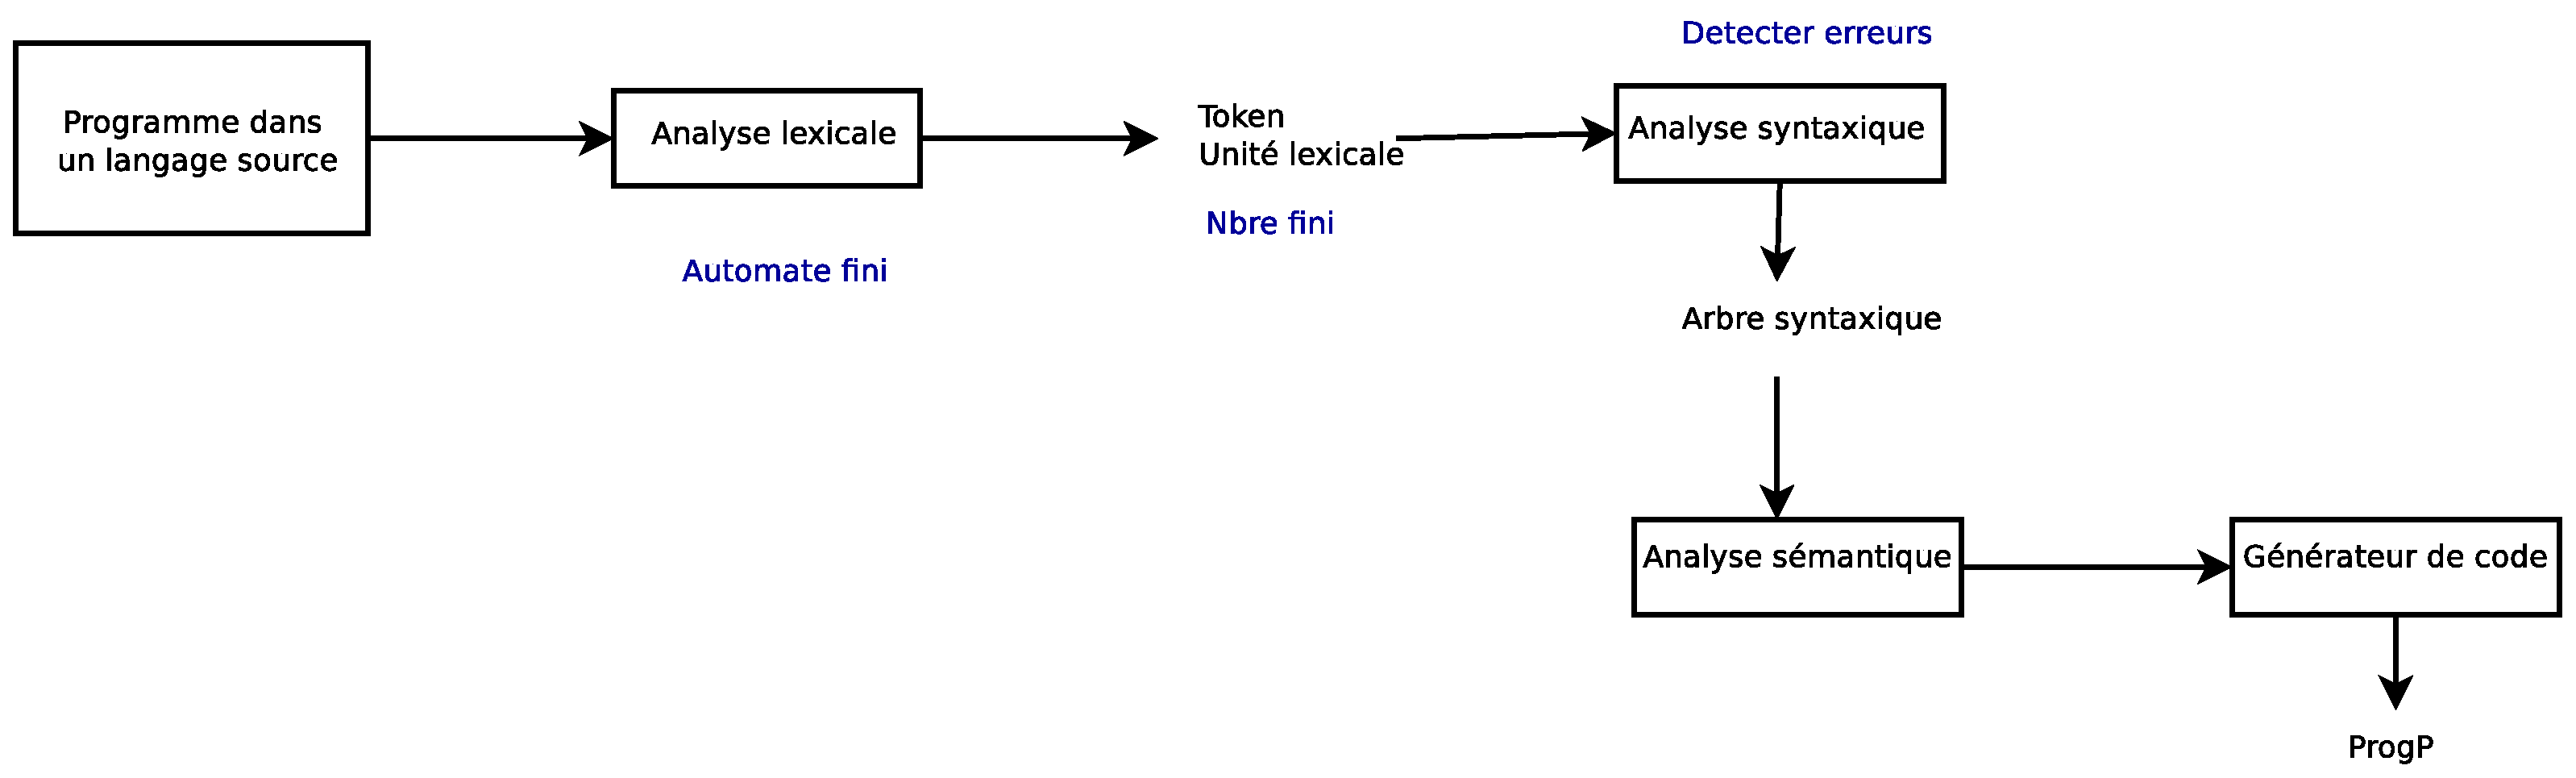
\includegraphics[width=19cm]{Diagramme3.eps}
		\caption{Phases de compilation}
	\end{figure}

	\chapter{Analyse lexicale}
	Un analyseur lexical doit découper un texte source en \tokens, l'analyseur lexicale peut aussi être appelé scanner. L'analyseur lexical ne
	fonctionne pas tout seul, il est en général guidé par un analyseur syntaxique.
	% Diag 4
	\begin{figure}[H]
		\centering
		\includegraphics[width=12cm]{Diagramme4.eps}
		\caption{Diagramme de traduction}
	\end{figure}

	\section{Token}
	\begin{itemize}
		\item Identificateur
		\item Mots clés
		\item Constantes numériques
		\item Opérateurs arithmétiques
		\item Opérateurs de comparaison
		\item Séparateur
		\item Commentaires
		\item Séparateurs
	\end{itemize}
	\section{Identificateurs}
	\begin{itemize}
		\item Commence par une lettre
		\item Suivi d'une suite éventuellement vide de lettres, de chiffres (et de caractères spéciaux)
	\end{itemize}
	\begin{description}
		\item[Nombres entiers signés]2014, +2014, -2014
		\item[Alphabet] $X=\{a,\cdots,z,\cdots 0,\cdots,9,(+),(-)\}$
	\end{description}

	\begin{exemple}
		\paragraph{Automate fini qui reconnait identificateurs et nombres}
		\begin{eqnarray*}
			L_0 &=&  l(L+c)^* + cc^* + (+) cc^* +(-)cc^*\\
			L_0 &=& 
		\end{eqnarray*}
	\end{exemple}

	\section{Fonctionnement}
	L'analyseur lexicale lit le texte caractère par caractère, découpe et reconnait des tokens(lexèmes) exprimé avec une regex.

	Il existe des outils générateurs de scanner.

	\subsection{Les problèmes posés par l'analyse lexicale}
	\subsubsection{Reconnaissance}
	Si on a \texttt{let} en mot clé et on a un identificateur \texttt{lettre}. On donne la priorité à l'unité syntaxique la plus longue, cf figure
	\ref{fig:recoPb} 

	\begin{figure}[H]
		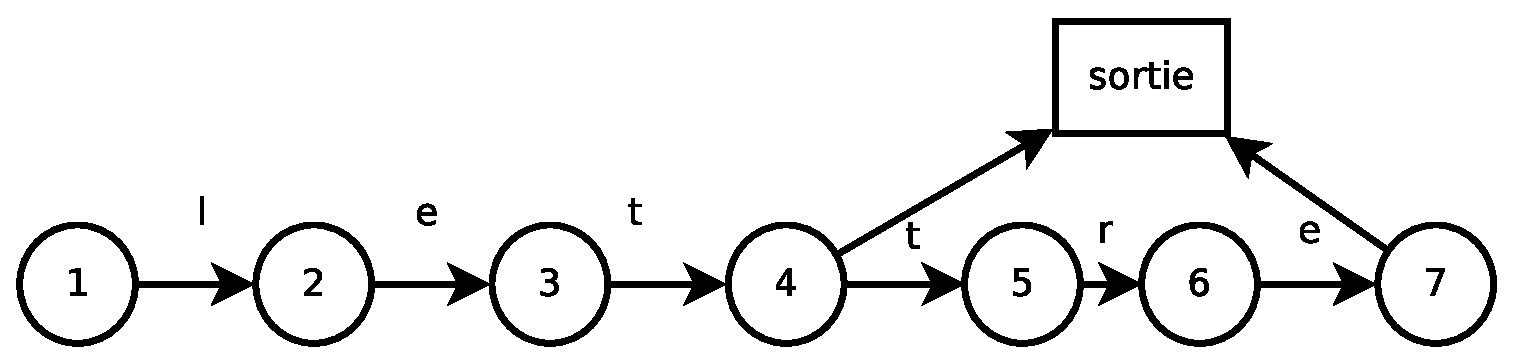
\includegraphics[width=12cm]{Diagramme5.eps}
		\centering
		\label{fig:recoPb}
	\end{figure}
	\subsubsection{Sur langage}
	Éventualité de faire un automate plus petit qui reconnait $L'$ tel que $L\subseteq L'$\footnote{C'est-à-dire un sur langage de $L$} avec des actions
	sémantiques plus << importantes >>.

	\subsubsection{Le recul}
	Si on a $<$, on sait que l’unité syntaxique c’est $<$. Mais si on tombe sur $<=$ on a une autre unité syntaxique ; $\leq$.

	Ce n'est pas réellement un problème car on a vu qu'on privilégie l'Unité Syntaxique(US) la plus longue.
	Si on tombe sur $<$ 1 , il faut remettre 1 dans le flot d’entrée

	\subsection{La table des symboles}
	La table des symboles, appelé TDS, est un endroit où ranger les \tokens rencontrés avec toutes les informations associées. Cela permet de calcul le <<
	hashcode>> pour la gestion des synonymes.

	\chapter{Analyse syntaxique}
	\paragraph{Objectif} Voir si les \tokens trouvés par l'AL forment une << phrase correcte>> ou non par rapport à la grammaire du langage.

	L'analyseur syntaxique est une grammaire reconnue par un automate à pile.

	\section{Analyse descendante}
Reconnaître(ou pas) un mot $u \in X^*$ sur le ruban, on part de $S$ et on a la pile.

À un instant donné, on a travaillé et on a reconnu un préfixe $\omega$ de u, $\omega \in X^*$.
Pour ça on a mis $A\alpha$ dans la pile, $A \in N$

A est le sommet de pile et $\alpha \in (N \cup X)^*$
	\chapter{Génération de code}
	On veut traduire les instructions du langage de haut niveau $L_1$ dans un
	langage intermédiaire plus proche du langage cible. On a 3 langages:
	\begin{itemize}
		\item Pour $L_1$ c’est un langage impératif composé de l'affectation, et toutes les structures de 
			contrôle(\texttt{if}, \texttt{else}, \texttt{case}, \texttt{switch}, \ldots) et des boucles (\texttt{for},
			\texttt{while}, \texttt{repeat}, \ldots)
		\item Pour $L_2$ (langage intermédiaire) on prend un langage de quadruplets. (choix)
		\item Pour $\sigma$, on va utiliser un langage impératif style ADA, Pascal
			Traduction $\sigma$ tq $\forall$ programme $P$ , $\forall$ donnée $PD \equiv \sigma(P)D$
	\end{itemize}

	\section{Langage intermédiaire des quadruplets}
	Nous avons un langage cible intermédiaire, qui ne ressemble pas vraiment à l'assembleur.\\
	Les opérations se font directement en mémoire, pas de registres. Un quadruplet est une instruction à 4 champs dont 3 adresses mémoire: 
	opération, opérande1, opérande2, résultat.

	On peut faire l'affectation, les opérations arithmétiques, les branchements conditionnels ou inconditionnels.
	\begin{description}
		\item[Affectation] \texttt{(:=, d, nil, e)}
		\item[Opération Arithmétique] \texttt{(+, a, b, c)}
		\item[Branchemnet inconditionnel] \texttt{(goto, nil, nil @)} 
	\end{description}

	\begin{lstlisting}[language=Algo, caption=Exemple de quadriplets]
@i		+, a, b, t1 -- t1 := a + b
@i+1	*, t1, c, t2 -- t2 := c * 1
@i+2	:=, t2, nil, d -- d := t2
@i+3	>?, a, b, alpha1 -- si a > b aller en alph1 sinon faire suivant
	\end{lstlisting}
	\section{Actions sémantiques couplées à l'analyseur descendant}
	L'analyseur syntaxique c’est le chef d’orchestre. Il est descendant et $LL(1)$

	Il s’occupe de l'analyse lexicale(AL) et de faire les actions sémantiques.
	\begin{itemize}
		\item Il va engendrer un programme équivalent en quadruplets.
			\begin{attention}
				Il n'y a pas d'exécution !
			\end{attention}
		\item Pour ça on va avoir besoin d’informations à mémoriser ou à modifier.
		\item Les procédures de descente récursive vont avoir besoin de paramètres en entrée ou en sortie et de variables locales.
	\end{itemize}

	\begin{exemple}
		Les expressions arithmétiques définies par la grammaire suivante :
		\begin{eqnarray*}
			E &\rightarrow& T\{+T\}*\\
			T &\rightarrow& F\{*F\}*\\
			F &\rightarrow& ident|(E)
		\end{eqnarray*}
		Notons que le symbole * sert ici pour le langage et pour définir l'opérateur de multiplication.
\begin{lstlisting}[language=Algo, framerule=0pt,  numbers=none]
Procedure E is
begin
	T;
	while NEXTS = '+' loop
		SKIP('+');
		T;
		-- * => engendre un quadruplet boite a outils
		GEN(QUAD: String);
		-- engendre le prochain quadruplet (A,B,C,D)
		GEN("+, ?, ?, ?")
	endloop 
end -- E
\end{lstlisting}
Il faut ajouter des arguments aux procédures E et T : $E \rightarrow T\{+T\}*$
\begin{lstlisting}[language=Algo, framerule=0pt,  numbers=none]
Procedure E (out r :String) is u, t :String;
begin
	T(r);
	while NEXTS = '+' loop
		SKIP('+');
		T(t); --2e operande
		u := NEWTEMP; -- Permet de créer une variable temporaire
		GEN("+","^r^", "^t^", "^u"); -- ^ est la concaténation 
		r := u;
	endloop
end //E
\end{lstlisting}
%% TODO NEXT p34
	\end{exemple}
	\section{Méthodologie pour la traduction des structures de contrôle}
	Traduction dirigée par la syntaxe, en un seul passage(lecture) du programme. Pour le moment, l'analyseur est descendant $LL(1)$. Il y a 3 étapes
	: 
	\begin{itemize}
		\item Donner le schéma en quadruplets correspond à la structure de contrôle traduite. Donner la sémantique de la structure de controle en quadruplets. ie ce qu'on veut savoir
		\item Donner l'inventaire des problèmes qui peuvent apparaitre et leurs solutions
		\item Écrire les procédures de traduction pour obtenir le schéma en quadruplets, ie comment on fait pour y arriver.
	\end{itemize}
	Pour ça, on a la boite à outils

	\appendix
	\chapter{Rappels}
	\section{Grammaire}
	Une grammaire est fait pour raconter de quelle manières les mots du langages sont construit. On part de l'axiome S et on applique les règles de
	productions, ou réécriture.

	Une grammaire $G=<N,X,P,S>$ avec : 
	\begin{description}
		\item[N] L'ensemble des non terminaux. Majuscules. $\{A,S,B\}$
		\item[X] Alphabet, ensemble des terminaux. Minuscules $\{a,b,c\}$
		\item[P] Règles de productions. À gauche on a un seul non terminal $P\{A \rightarrow \alpha, A\in N, \alpha\in(N \cup X)\}$ 
		\item[S] $S\in N$ Axiome 
	\end{description}
	~

	\begin{exemple}
		\begin{eqnarray*}
			G_1&=& <N,X,P,S>\\
			N&=& \{S\}\\
			X&=& \{a,b\}\\
			P&=& \{S \rightarrow abS, S\rightarrow a\}
		\end{eqnarray*}
	\end{exemple}
	\begin{exemple}
		\begin{eqnarray*}
			G_2 &=&  <N,X,P,S>\\
			N &=& \{S,A\}\\
			X&=& \{a,b,c\}\\
			P&=& \{S \rightarrow aAc\\
			&& \ A\rightarrow bbA\\
			&& \ A\rightarrow b\}
		\end{eqnarray*}
	\end{exemple}

	$\omega \in X^*$ est un mot engendré par G, $\Rightarrow \omega \in L(G)$, avec $L(G)$ qui est un langage engendré par G.

	\begin{exemple}
		Avec $G_1$ : 
		$S \Rightarrow abS \Rightarrow ababS \Rightarrow ababa\in L(G_1)$
	\end{exemple}

	\subsection{Théorèmes}
	\subsubsection{Théorème d'Arden}
	$P$ règle de production $G$, système d'équation de langages, c'est à dire résoudre L(G).

	$X =  r_1 X + r_2 \Rightarrow X = r_1\* r_2$ est solution. Si $\lambda \not\in r_1$ alors la solution est unique.
	\begin{exemple}
		\begin{eqnarray*}
			G_1 &\leadsto& S = \underbrace{ab}_{r_1}S + \underbrace{a}_{r_2}\\
			G_2 &\leadsto& \left\{\begin{array}{ccc} S& =& aAc\\
				A& =& \underbrace{bb}_{r_1}A+\underbrace{b}_{r_2}\end{array}\right.
			\end{eqnarray*}
		\end{exemple}

		\subsubsection{Théorème d'Arden bis}
		$$X = Xr_1+r_2 \Rightarrow X=r_2r_1^{\;*}$$

		\subsubsection{Théorème $A^nB^n$}
		$$X = YXZ+T \Rightarrow X = Y^nTZ^n$$

		\section{Reconnaître un langage avec un automate à pile}
		Un automate à pile est défini par $<Q,X,q_0,\Gamma, Z_0,F$
		\begin{description}
			\item[Q] Ensemble d'état
			\item[X] Alphabet
			\item[$q_0 \in Q$] Etat initial
			\item[$\Gamma$] Alphabet de pile
			\item[$Z_0$] Fond de pile $Z_0 \in \Gamma$
			\item[F] Ensemble d'états finales $F\subseteq Q$
			\item[$\sigma$] Fonction de transition 
		\end{description}

		\begin{exemple}
			\begin{eqnarray}
				S &\rightarrow& aAc\\
				A &\rightarrow& bbA \\
				A &\rightarrow& b \\
				N &=& S,\\
				X &=& a, b, c\\
				\sigma(q, \lambda, S)& =& (q, aAc) \\
				\sigma(q, \lambda, A) &=& (q, bbA)\\
				\sigma(q, \lambda, A) &=& (q, b)\\
				\sigma(q, a, a) &=& (q, \lambda)\\
				\sigma(q, b, b) &=& (q, \lambda)\\
				\sigma(q, c, c) &=& (q, \lambda)
			\end{eqnarray}

			\begin{center}
				Analyse de la séquence abbbbbc

				\begin{tabular}{ccc}
					\textbf{Ruban} & \textbf{Pile} & \textbf{Règle}\\
					\hline
					$\lambda abbbbbc$ &$S$ &A.6\\
					$abbbbbc$ &$aAc$& A.9\\
					$\lambda bbbbbc$ &$Ac$ &A.7\\
					$\lambda bbbbbc$ &$bbAc$& A.10\\
					$bbbbc$ &$bAc$& A.10\\
					$bbbc$ &$Ac$ &A.7\\
					$bbbc$ &$bbAc$& A.10\\
					$bbc$& $bAc$& A.10\\
					$\lambda bc$&$ Ac$& A.8\\
					$bc$& $bc$& A.10\\
					c &$c$& A.11\\
					mot lu &pile vide&
				\end{tabular}
			\end{center}

			L'analyse doit se faire en une seule lecture du ruban et de façon déterministe. 

			Pour cela, on regarde $k$ symboles sur le ruban pour pouvoir décider de façon unique de la règle à appliquer. 
			Cette analyse efficace est appelée analyse k-prédictive.

			On peut écrire un algo déterministe pour la reconnaissance de $\omega \in L(G_2 )$
			\begin{lstlisting}[language=C,numbers=none]
				Utiliser A.6;
				Utiliser A.9 pour dépiler "a"
				while il y a "bb" sur le ruban, do:
				Utiliser A.7;
				Utiliser deux fois A.10 pour dépiler les 2 "b"
				end
			\end{lstlisting}
		\end{exemple}
		\listoffigures

		\end{document}

